\normaltrue
\correctionfalse

%\UPSTIidClasse{11} % 11 sup, 12 spé
%\newcommand{\UPSTIidClasse}{12}

%\section{Rotation simple} %\label{B2:12:01}
\exer{Mouvement R  $\star$ \label{B2:13:02}}
\setcounter{question}{0}
\UPSTIcompetence[2]{B2-13}

\index{Compétence B2-13}
\index{Mécanisme à 1 rotation}
\ifcorrection
\else
\marginnote{\textbf{Pas de corrigé pour cet exercice.}}
\fi

\ifprof
\else
Soit le mécanisme suivant. On a $\vect{AB}=R\vect{i_1}$ avec $R=\SI{20}{mm}$. 
\begin{center}
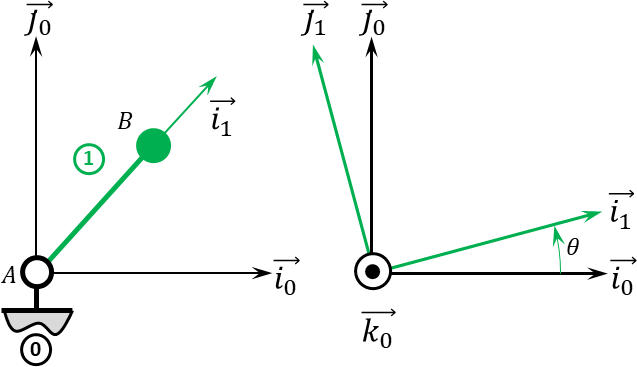
\includegraphics[width=\linewidth]{02_R_01}
\end{center}
\fi

\question{Déterminer $\vectv{B}{1}{0}$ par dérivation vectorielle ou par composition.}
\ifprof
\else
\fi

\question{Donner le torseur cinématique $\torseurcin{V}{1}{0}$ au point $B$.}
\ifprof
\else
\fi

\question{Déterminer $\vectg{B}{1}{0}$.}
\ifprof
\else
\fi


\ifprof
\else
\begin{flushright}
\footnotesize{Corrigé  voir \ref{B2:13:02}.}
\end{flushright}%
\fi